%!TEX root=RKWard_paper.tex
\section{Technical design}
\label{sec:technical}
In this section we will give a compact overview of the key aspects of RKWard's
technical design. We will give slightly more attention to the details of the
plugin framework (Section~\ref{sec:technical_plugins}) used in RKWard, since this is central to the extensibility of
RKWard.

\subsection{Asynchronous command execution}
\label{sec:technical_asynchronous}
One central design decision in the implementation of RKWard is that the
interface to the \proglang{R} engine operates asynchronously. The intention is to
keep the application usable to a high degree, even during the computation of
time-consuming analysis. For instance, while waiting for the estimation of a
complex model to complete, the user should be able to continue to use the GUI to
prepare the next analysis. Asynchronous command execution is also a prerequisite
for an implementation of the plot-preview feature (see Section~\ref{sec:plot_previews}). Commands
generated from plugins or user actions are placed in queue and are evaluated in
a separate thread in the order they were submitted\footnote{
    It is possible, and in some cases necessary, to enforce a different order of command execution in
    internal code. For instance, RKWard makes sure that no user command can
    potentially interfere while RKWard is loading the data of a \code{data.frame} for
    editing.
}. The asynchronous design implies that RKWard avoids relying on the
\proglang{R} engine during interactive use. This is one of several reasons for
the use of \proglang{ECMAScript} in plugins, instead of scripting using
\proglang{R} itself (see Sections~\ref{sec:technical_toolkit} and \ref{sec:technical_plugins}).
A further implication is that RKWard avoids querying information about the
existence and properties of objects in \proglang{R} interactively. Rather,
RKWard keeps a representation of \proglang{R} objects and their basic properties
(e.\,g., class and dimensions), which is used for the workspace browser (Section~\ref{sec:workspace_browser_object_viewer}),
object name completion, function argument hinting, and
other places. The object representation includes objects in all environments
in the search path, and any objects contained within these environments in a
hierarchical tree\footnote{
    Currently, environments of functions or formulas are not taken into account.
}. The representation of \proglang{R} objects is gathered
pro-actively. This has a notable impact on performance when loading packages.
Specifically, objects which would usually be ``lazy loaded'' only when needed \citep[see][]{Ripley2004} are
accessed in order to fetch information on their properties. This means the data
has to be loaded from disk; however, the memory is freed immediately after fetching
information on the object. Additionally, for packages with extremely large number of objects, RKWard
provides an option to exclude specific packages from scanning the object structures.

A further side-effect of the asynchronous threaded design is that there is
inherently a rather clear separation between the GUI code and the code making direct use
of the \proglang{R} application programming interface (API) (see also Figure~\ref{fig:design_sketch}). 
In the current development version, the evaluation
of \proglang{R} commands has even been moved into a separate process. Therefore in future releases it could 
be made possible to run GUI and \proglang{R} engine on different computers.

\begin{figure}[t!]
 \centering
 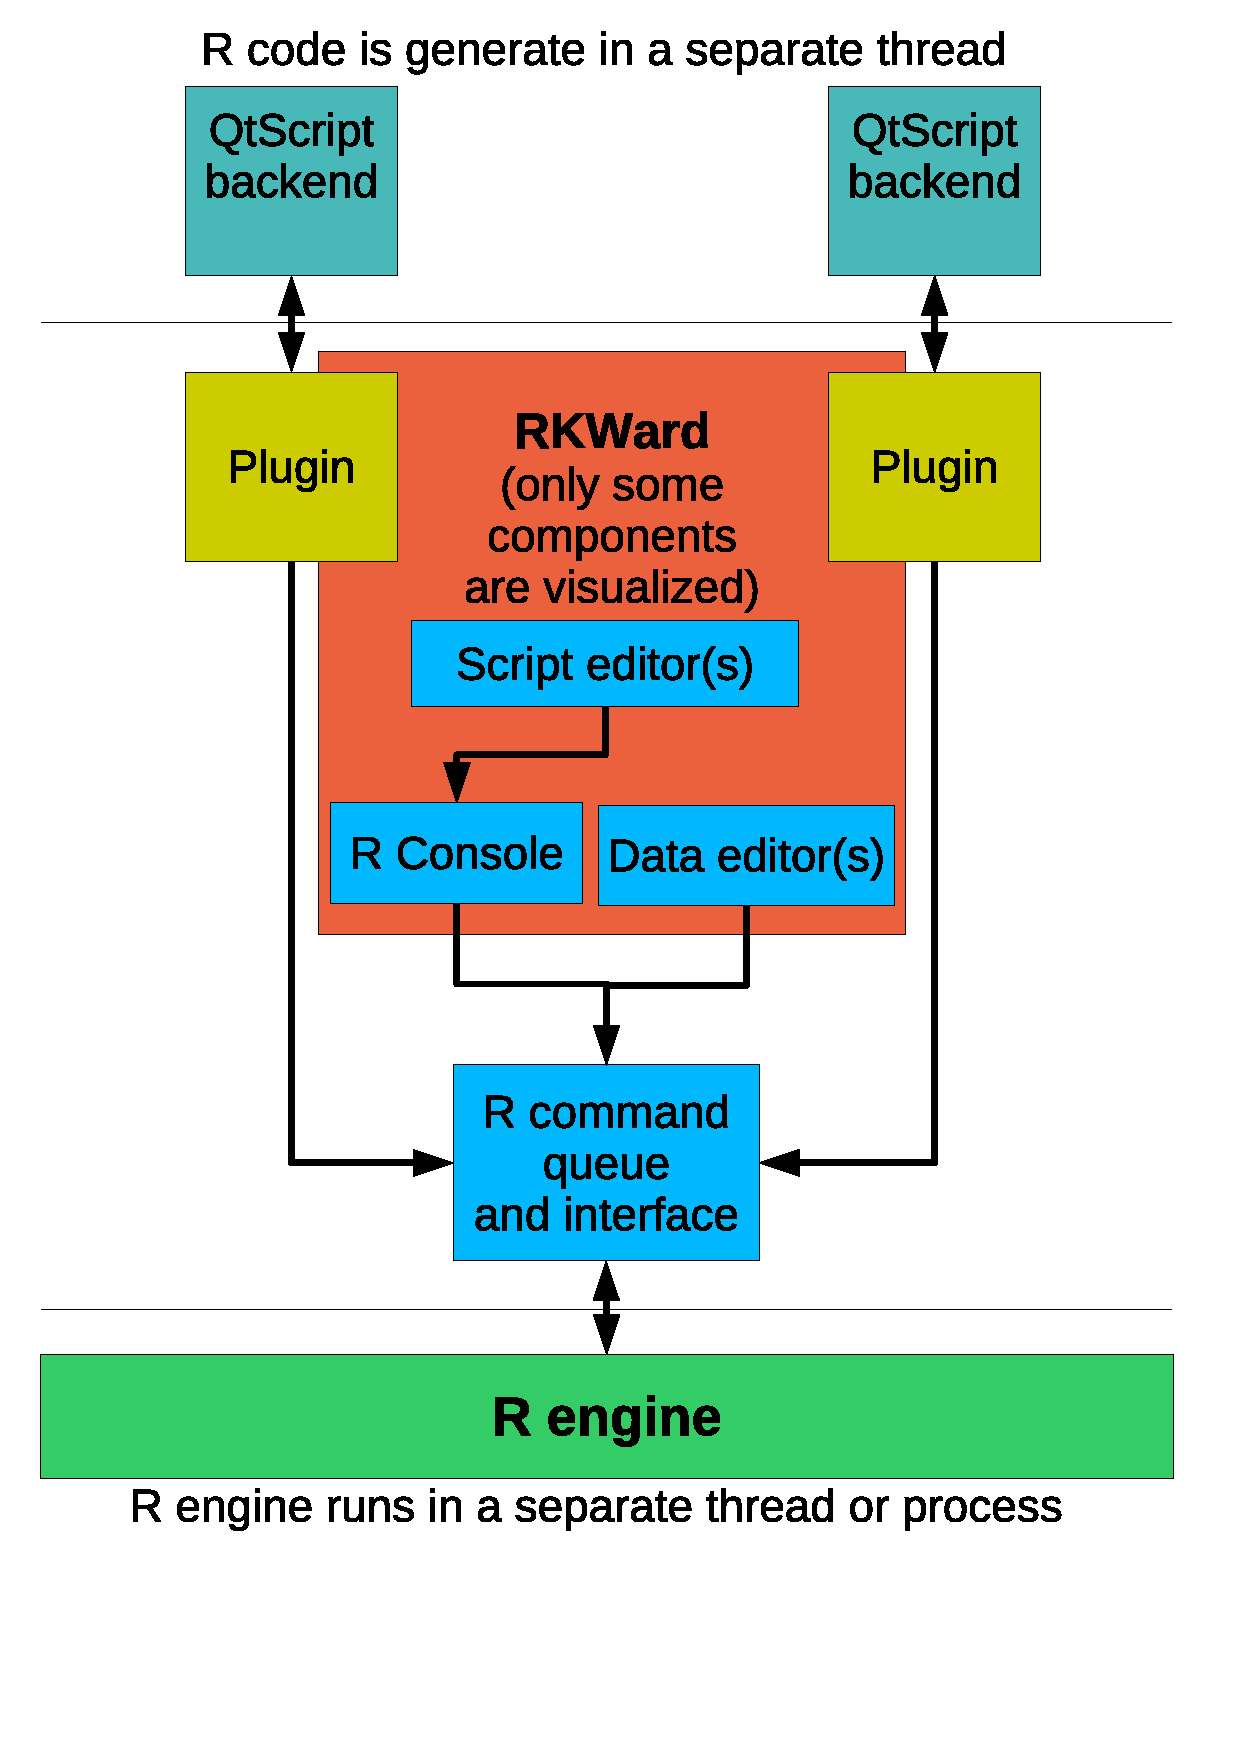
\includegraphics{../figures/design_sketch.pdf}
 \caption{Technical design of RKWard. Only a few central components are visualized.
 All communication with the \proglang{R} engine is passed through a single interface living in the main application thread. The \proglang{R} engine itself
 runs in a separate thread (or in a separate process). 
 Separate threads are also used to generate \proglang{R} code from plugins.
}
 \label{fig:design_sketch}
\end{figure}

\subsection{Object modification detection}
\label{sec:technical_omd}
RKWard allows the user to run arbitrary commands in \proglang{R} at any time, even while
editing a \code{data.frame} or while selecting objects for analysis in a GUI dialog. Any user
command can potentially add, modify, or remove objects in \proglang{R}. RKWard tries to
detect such changes in order to always display accurate information in the
workspace browser, object selection lists, and object views. Beyond that,
detecting any changes is particularly important with respect to objects which
are currently being edited in the data editor (which provides an illusion
of in-place editing, see Section~\ref{sec:spreadsheet}). Here, it is necessary to synchronize
the data between \proglang{R} and the GUI in both directions.

For simplicity and performance, object modification detection is only
implemented for objects inside the ``global environment'' (including environments
inside the global environment), since this is where changes are typically done.
Currently, object modification detection is based on active bindings.
Essentially, any object which is created in the global environment is first
moved to a hidden storage environment, and then replaced with an active binding.
The active binding acts as a transparent proxy to the object in the storage
environment, which registers any write-access to the object\footnote{
    This is similar to the approach taken in the \pkg{trackObjs} package \citep{Plate2009}.
}.

The use of active bindings has significant performance implications when
objects are accessed very frequently. This is particularly notable where an
object inside the global environment is used as the index variable in a loop,
as illustrated by the following example. When control returns to the top level
prompt, after the first assignment, \code{i} will become subject to object modification
detection (i.\,e., it will be wrapped into an active
binding). The subsequent \code{for} loop will then run slow.

\begin{Code}
R> i <- 1
R> for (i in 1:100000) i + i
\end{Code}

In contrast, in the following example, \code{i} is a local object, and will not
be replaced by an active binding. Therefore the loop will run approximately as fast
as in a plain \proglang{R} session:

\begin{Code}
R> f <- function () {
R+    i <- 1
R+    for (i in 1:100000) i + i
R+ }
R> f ()
\end{Code}

Future versions of RKWard will try to avoid this performance problem. 
One approach that is currently under consideration is to simply perform
a pointer comparison of the SEXP records of objects in global environment with
their copies in a hidden storage environment. Due to the implicit sharing of
SEXP records \citep{RDCT2010a, RDCT2010b}, this should provide for a reliable
way to detect changes for most types of \proglang{R} objects, with comparatively low memory
and performance overhead. Special handling will be needed for environments and
active bindings.

\subsection{Choice of toolkit and implementation languages}
\label{sec:technical_toolkit}
In addition to \proglang{R}, RKWard is based on the \proglang{KDE} libraries, which are in turn based
on \proglang{Qt}, and implemented mostly in \proglang{C++}. Compared to many competing libraries,
this constitutes a rather heavy dependency. Moreover, the \proglang{KDE} libraries are
still known to have portability issues especially on Mac OS X, and to some degree
also on the Windows platform.

The major reason for choosing the \proglang{KDE} and \proglang{Qt} libraries was their 
many high level features which have allowed RKWard development to make quick
progress despite limited resources. Most importantly, the \proglang{KDE} libraries provide a
full featured text editor \citep{CullmannND} as a component which can be
seamlessly integrated into a host application using the KParts technology
\citep{Faure2000}. Additionally, another KPart provides \proglang{HTML} browsing capabilities in a
similarly integrated way. The availability of KWord \citep{KWord} as an
embeddable KPart might prove useful in future versions of RKWard, when better
integration with office suites will be sought.

Another technology from the \proglang{KDE} libraries that is important to the development
of RKWard is the ``XMLGUI'' technology
\citep{Faure2000}. This is especially helpful in providing an integrated GUI across
the many different kinds of document windows and tool views supported in RKWard.

Plugins in RKWard rely on \proglang{XML} (extensible markup language)\footnote{\url{http://www.w3.org/XML/}}
and \proglang{ECMAScript}\footnote{\url{http://www.ecmascript.org/}} (see Section~\ref{sec:technical_plugins}). \proglang{XML} is not
only well suited to describe the layout of the GUI of plugins, but simple
functional logic can also be represented \citep[see also][]{Visne2009}. \proglang{ECMAScript} was
chosen for the generation of \proglang{R} commands within plugins, in particular due to its
availability as an embedded scripting engine inside the \proglang{Qt} libraries. While at
first glance \proglang{R} itself would appear as a natural choice of scripting language as
well, this would make it impossible to use plugins in an asynchronous way.
Further, the main functional requirement in this place is the manipulation and
concatenation of text strings. While \proglang{R} provides support for this, concatenating
strings with the \code{+}-operator, as available in \proglang{ECMAScript}, allows for a much
more readable way to perform such basic text manipulation.

\subsection{On-screen graphics windows}
\label{sec:technical_graphics}
Contrary to the approach used in \pkg{JGR} \citep{JGR2010}, RKWard does
not technically provide a custom on-screen graphics device. RKWard detects when
new graphics windows are created via calls to \code{X11()} or \code{windows()}. These windows
are then ``captured'' in a platform dependent way (based on the XEmbed \citep{Ettrich2002} protocol
for X11, on reparenting for the Windows platform). An RKWard menu bar and a
toolbar is then added to these windows to provide added functionality. While
this approach requires some platform dependent code, any corrections or
improvements made to the underlying \proglang{R} native devices will automatically be
available in RKWard.

A recent addition to the on-screen device is the ``plot history'' feature which
adds a browsable list of plots to the device window. Since RKWard does not use a
custom on-screen graphics device, this feature is implemented in a package
dependent way. For example, as of this writing, plotting calls that use either
the ``standard graphics system'' or the ``\pkg{lattice} system'' can be added to the plot
history; other plots are drawn but not added. The basic procedure is to identify
changes to the on-screen canvas and record the existing plot before a new plot
wipes it out. A single global history for the recorded plots is maintained
which is used by all the on-screen device windows. This is similar to the
implementation in \proglang{Rgui.exe} (Windows), but unlike the one in \proglang{Rgui.app} 
(Mac OS X). Each such device window points to a position in the history
and behaves independently when recording a new plot or deleting an existing
one.

The \pkg{lattice} system is implemented by inserting a hook in the \code{print.lattice()}
function. This hook retrieves and stores the \code{lattice.status} object from the
\code{lattice:::.LatticeEnv} environment, thereby making \code{update()} calls on trellis
objects transparent to the user. Any recorded trellis object is then replayed
using \code{plot.lattice()}, bypassing the recording mechanism. The standard graphics
system, on the other hand, is implemented differently because the hook in
\code{plot.new()} is ineffective for this purpose. A customized function is overloaded
on \code{plot.new()} which stores and retrieves the existing plot, essentially, using
\code{recordPlot()} and replays them using \code{replayPlot()}.

The actual plotting calls are tracked using appropriate \code{sys.call()} commands in
the hooks. These call strings are displayed as a drop-down menu on the toolbar
for non-sequential browsing (see Figure~\ref{fig:plot_history}) providing a very intuitive browsing
interface unlike the native implementations in \code{windows()} and \code{quartz()} devices.

\subsection{Plugin infrastructure}
\label{sec:technical_plugins}
One of the earliest features of RKWard was the extensibility by plugins.
Basically, plugins in RKWard provide complete GUI-dialogs, or re-usable
GUI-components, which accept user settings and translate those user settings
into \proglang{R} code\footnote{
    Plugins are also used in some other contexts within RKWard, for instance, the
    integrated text editor (kate part) supports extensions via plugins and user scripts. At this point we
    will focus only on plugins generating \proglang{R} code.
}. Thus, the plugin framework is basically a tool set used to define
GUIs for the automatic generation of \proglang{R} code.

Much of the functionality in RKWard is currently implemented as plugins. For example, importing different file
formats relying on the \pkg{foreign} package is achieved by this approach. Similarly,
RKWard provides a modest GUI driven tool set for statistical analysis,
especially for item response theory (IRT), distributions, and descriptive
statistical analysis.

\subsubsection{Defining a plugin}
\label{sec:technical_plugins_defining}
Plugins consist of four parts as visualized in Figure~\ref{fig:plugin_structure} 
\citep[see Section~\ref{sec:example_plugin} for an example; for a complete
manual, see][]{Friedrichsmeier2010}:

\begin{figure}[b!]
 \centering
 \includegraphics[width=8cm]{../figures/plugin_structure.pdf}
 \caption{Plugin structure of RKWard. One or more plugins are declared in a ``plugin map''. Each plugin is defined by
 two \proglang{XML} files, and one \proglang{ECMAScript} file.}
 \label{fig:plugin_structure}
\end{figure}

\begin{itemize}
    \item
    An \proglang{XML} file (Section~\ref{sec:defining_menu_hierarchy}), 
    called a ``plugin map'', is used to declare one or more plugins, each
    with a unique identifier. For most plugins, the plugin map also defines the
    placement in the menu hierarchy. Plugin maps are meant to represent groups of
    plugins. Users can disable/enable such groups of plugins in order to reduce the
    complexity of the menu hierarchy.

    \item
    A second \proglang{XML} file describes the plugin GUI layout itself (Section~\ref{sec:defining_dialog_ui}). 
    Most importantly this includes
    the definition of the GUI-layout and GUI-behavior. High level GUI-elements can
    be defined with simple \proglang{XML}-tags. Layout is based on ``rows'' and ``columns'',
    instead of pixel counts. In most cases this allows for a very sensible resizing
    behavior. RKWard supports single-page dialogs and multi-page wizards, however,
    most plugins define only a single-page GUI. GUI behavior can be programmed by
    connecting ``properties'' of the GUI elements to each other. For example, the state
    of a checkbox could be connected to the ``enabled'' property of a dependent
    control. More complex logic is also supported, as is procedural scripting of GUI
    behavior using \proglang{ECMAScript}.

    \item
    A separate \proglang{ECMAScript} file (Section~\ref{sec:generating_r_code_from_ui_settings}) 
    is used to translate GUI settings into \proglang{R}
    code\footnote{
        In earlier versions of RKWard, \proglang{PHP} was used
        as a scripting engine, and \proglang{PHP} interpreters were run as separate processes.
        Usage of \proglang{PHP} was abandoned in RKWard version 0.5.3 for reasons of performance and simplicity.
    }. This \proglang{ECMAScript} file is evaluated asynchronously in a separate thread. RKWard
    currently enforces structuring the code into three separate sections for
    preprocessing, calculating, and printing results. The generated code is always
    run in a local environment, in order to allow the use of temporary variables
    without the danger of overwriting user data.

    \item
    A third \proglang{XML} file defines a help page. This help page usually links to the \proglang{R} help
    pages of the main functions/concepts used by the plugin, as well as to other 
    related RKWard help pages. Compared to \proglang{R} help
    pages, the plugin help pages try to give more hands-on advice on using the
    plugin. Plugins can be invoked from their help page by clicking on a link near
    the top, which can be useful after following a link from a related help page.
\end{itemize}

Changes to the source code of these elements take effect without the requirement to recompile RKWard.

\subsubsection{Embedding and reuse of plugins}
\label{sec:technical_plugins_embedding}
RKWard supports several mechanisms for modularization and re-use of
functionality in plugins. File inclusion is one very simple but effective
mechanism, which can be used in the \proglang{ECMAScript} files, but is also supported in
the \proglang{XML} files. In script files, this is most useful by defining common functions
in an included file. For the \proglang{XML} files, the equivalent is to define ``snippets''
in the included file, which can then be inserted.

A third mechanism allows to completely embed one plugin into another. For
instance the \code{plot\_options} plugin is used by many plugins in RKWard, to provide
common plot options such as labels, axis options, and grids. Other plugins
can embed it using the \code{embed}-tag in their \proglang{XML} file (the plugin supports
hiding irrelevant options). The generated code portions can be fetched from the
\proglang{ECMAScript} file just like any other GUI settings, and inserted into the complete
code. Other examples of embedded plugins are options for histograms, barplots,
and empirical cumulative distribution function (ECDF) plots (which in turn embed the generic plot options plugin).

\subsubsection{Enforcing a consistent interface}
\label{sec:technical_plugins_consistency}
RKWard tries to make it easy to create a consistent interface in all plugins.
GUI-wise this is supported by providing high-level GUI elements, and embeddable
clients. Also, the standard elements of each dialog (``Submit'', and
``Cancel'' buttons, on-the-fly code view, etc.) are hard coded. Up to version
0.5.3 of RKWard it was not possible to use any GUI elements in plugins which
were not explicitly defined for this purpose. In the current development
version, theoretically, all GUI elements available from \proglang{Qt} can be inserted,
where necessary.

For generating output, the function \code{rk.header()} can be used to print a
standardized caption for each piece of output. Printing results in vector or
tabular form is facilitated by \code{rk.results()}. A wide range of objects can be
printed using \code{rk.print()}, which is just a thin wrapper around the
\code{HTML()} function of the \pkg{R2HTML} package \citep{Lecoutre2003} in the current
implementation. The use of custom formatting with \proglang{HTML} is possible, but
discouraged. Standard elements such as a horizontal separator, and the ``Run again''
link (see Section~\ref{sec:results_output}) are inserted automatically, without the need to define
them for each plugin.

Regarding the style of the generated \proglang{R} code, enforcing consistency is harder,
but plugins which are to become part of the official RKWard application are
reviewed for adherence to some guidelines. Perhaps the most important guidelines
are 

\begin{itemize}
  \item 
  Write readable code, which is properly indented, and commented where necessary.

  \item 
  Do not hide any relevant computations from the user by performing them in the
  \proglang{ECMAScript}. Rather, generate \proglang{R} code which will perform
  those computations, transparently.

  \item
  Plugins can be restricted to accept only certain types of data (such as only one-dimensional numeric data).
  Use such restrictions where appropriate to avoid errors, but be very careful not to add
  too many of them.
\end{itemize}

\subsubsection[Handling of R package dependencies]{Handling of \proglang{R} package dependencies}
\label{sec:technical_plugins_dependencies}
A wide range of plugins for diverse functionality is present in RKWard,
including plots (e.\,g., boxplot) or standard tests (e.\,g., Student's t-test)\footnote{
  At the time of this writing, there are 164 user-accessible plugins in RKWard.
  Listing all is beyond the scope of this article.
}. Some
of the plugins depend on \proglang{R} packages other than the recommended \proglang{R} base packages.
Examples herein are the calculation of kurtosis, skewness or the exact Wilcoxon
test.

RKWard avoids loading all these packages pro-actively, as \pkg{Rcmdr} does. Rather,
plugins which depend on a certain package simply include an appropriate call to
\code{require()} in the pre-processing section of the generated \proglang{R} code. The \code{require()}
function is overloaded in RKWard, in order to bring up the package-installation
dialog (see Section~\ref{sec:package_management}) whenever needed. Packages invoked by \code{require()} remain loaded
in the active RKWard session unless unloaded, manually (from the workspace browser, or using the
\proglang{R} function \code{detach()}).

Dependencies between (embedded) plugins are handled using the \code{<require>}-tag in the plugin map.

\subsection{Development process}
\subsubsection{RKWard core and external plugins}
\label{sec:technical_processes_plugins}
Newly developed plugins are placed in a dedicated plugin map file.
Plugins in this map are not visible to the user by
default, but need to be enabled manually. Once the author(s) of a plugin
announces that they consider it stable, the plugin is subjected to a review for
correctness, style, and usability. The review status is tracked in the project
wiki. Currently at least one positive review is needed before the plugin is
allowed to be made visible by default, by moving it to an appropriate plugin
map.

The current development version adds support for downloading additional sets of
plugins, which are neither officially included nor supported by the
RKWard developers, from the internet.

\subsubsection{Automated testing}
\label{sec:technical_processes_automatedtesting}
A second requirement for new plugins is that each plugin must be accompanied by
at least one automated test. The automated testing framework in RKWard consists
of a set of \proglang{R} scripts which allow to run a plugin with specific GUI settings,
automatically\footnote{
  In the current development version, the scripts have been converted into a proper
  \proglang{R} package.
}. The resulting \proglang{R} code, \proglang{R} messages, and output are then compared
to a defined standard. Automated tests are run routinely after changes in the
plugin infrastructure, and before any new release.

The automated testing framework is also useful in testing some aspects of the
application which are not implemented as plugins, but this is currently limited
to very few basic tests.

\subsection{Internationalization}
\label{sec:technical_internationalization}
Currently strings in the main application are translated to varying extents in
Czech (cs), Catalan (ca), Spanish (es), German (de), Chinese (zh\_CN), Turkish
(tr), Polish (pl), Italian (it), French (fr), Greek (el), and Danish (da).
Translatable strings are to be found under po/**.po in the sources. These files
can conveniently be edited with front-ends like Lokalize\footnote{\url{http://i18n.kde.org/tools/}}. 

Plugins and help pages in RKWard are not translatable at the time of this
writing. While it will be technically possible to include the respective strings in
message catalogs, this is not currently implemented in RKWard. Similarly, any
output generated by \proglang{R} functions defined for RKWard is not currently
translatable. Again, however, there is no technical barrier with respect to
internationalization of \proglang{R} code, as discussed by \cite{Ripley2005a},
and it is planned to make RKWard fully translatable in future versions.
